%% Copernicus Publications Manuscript Preparation Template for LaTeX Submissions
%% ---------------------------------
%% This template should be used for copernicus.cls
%% The class file and some style files are bundled in the Copernicus Latex Package, which can be downloaded from the different journal webpages.
%% For further assistance please contact Copernicus Publications at: production@copernicus.org
%% https://publications.copernicus.org/for_authors/manuscript_preparation.html


%% Please use the following documentclass and journal abbreviations for discussion papers and final revised papers.

%% 2-column papers and discussion papers
\documentclass[tc, manuscript]{copernicus}



%% Journal abbreviations (please use the same for discussion papers and final revised papers)


% Advances in Geosciences (adgeo)
% Advances in Radio Science (ars)
% Advances in Science and Research (asr)
% Advances in Statistical Climatology, Meteorology and Oceanography (ascmo)
% Annales Geophysicae (angeo)
% Archives Animal Breeding (aab)
% ASTRA Proceedings (ap)
% Atmospheric Chemistry and Physics (acp)
% Atmospheric Measurement Techniques (amt)
% Biogeosciences (bg)
% Climate of the Past (cp)
% DEUQUA Special Publications (deuquasp)
% Drinking Water Engineering and Science (dwes)
% Earth Surface Dynamics (esurf)
% Earth System Dynamics (esd)
% Earth System Science Data (essd)
% E&G Quaternary Science Journal (egqsj)
% Fossil Record (fr)
% Geochronology (gchron)
% Geographica Helvetica (gh)
% Geoscience Communication (gc)
% Geoscientific Instrumentation, Methods and Data Systems (gi)
% Geoscientific Model Development (gmd)
% History of Geo- and Space Sciences (hgss)
% Hydrology and Earth System Sciences (hess)
% Journal of Micropalaeontology (jm)
% Journal of Sensors and Sensor Systems (jsss)
% Mechanical Sciences (ms)
% Natural Hazards and Earth System Sciences (nhess)
% Nonlinear Processes in Geophysics (npg)
% Ocean Science (os)
% Primate Biology (pb)
% Proceedings of the International Association of Hydrological Sciences (piahs)
% Scientific Drilling (sd)
% SOIL (soil)
% Solid Earth (se)
% The Cryosphere (tc)
% Weather and Climate Dynamics (wcd)
% Web Ecology (we)
% Wind Energy Science (wes)


%% \usepackage commands included in the copernicus.cls:
%\usepackage[german, english]{babel}
%\usepackage{tabularx}
%\usepackage{cancel}
%\usepackage{multirow}
%\usepackage{supertabular}
%\usepackage{algorithmic}
%\usepackage{algorithm}
%\usepackage{amsthm}
%\usepackage{float}
%\usepackage{subfig}
%\usepackage{rotating}


\begin{document}

\title{DeepBedMap: Using a deep neural network to better resolve the bed topography of Antarctica}


% \Author[affil]{given_name}{surname}

\Author[1]{Wei Ji}{Leong}
\Author[1]{Huw}{Horgan}

\affil[1]{Antarctic Research Centre, Victoria University of Wellington, Wellington, New Zealand}

%% The [] brackets identify the author with the corresponding affiliation. 1, 2, 3, etc. should be inserted.


\correspondence{W. J. Leong (weiji.leong@vuw.ac.nz)}

\runningtitle{TEXT}

\runningauthor{TEXT}





\received{}
\pubdiscuss{} %% only important for two-stage journals
\revised{}
\accepted{}
\published{}

%% These dates will be inserted by Copernicus Publications during the typesetting process.


\firstpage{1}

\maketitle



\begin{abstract}
To better resolve the bed elevation of Antarctica, we present a novel deep convolutional neural network that produces realistic terrain given multiple remote sensing data inputs.
Our super-resolution DeepBedMap neural network model is trained on scattered regions in Antarctica where high resolution groundtruth bed elevation grids are available, and later used to generate high resolution bed topography in less well surveyed areas.
DeepBedMap improves on previous interpolation methods by not restricting itself to a low spatial resolution (1000m) BEDMAP2 raster image as its prior.
It takes in additional high spatial resolution datasets, such as Antarctic ice surface velocity and surface elevation maps, which can be used to better inform the bed topography even in the absence of direct ice-penetrating radar survey data.
Our DeepBedMap model is based on an adapted Enhanced Super Resolution Generative Adversarial Network architecture, chosen to minimize the per-pixel elevation error while producing realistic topography.
The final product is a four times upsampled (250m) bed elevation model of Antarctica that can be used by glaciologists interested in the subglacial terrain, and also ice sheet modellers wanting to run catchment or continent-scale ice sheet model simulations.
We show that DeepBedMap produces a more accurate digital elevation model than a baseline bicubic interpolation product, and also compare it with other synthetic bed elevation models on reference groundtruth survey tracks.
\end{abstract}


\copyrightstatement{This work is distributed under the Creative Commons Attribution 4.0 License}


\introduction  %% \introduction[modified heading if necessary]

In order to create a more detailed map of Antarctica's bed, we present a novel deep convolutional neural network that produces realistic terrain given multiple remote sensing data inputs.
A higher resolution digital bed elevation model of Antarctica enables us to better quantify glacier ice flow mechanics, particularly along fast flowing ice streams near the grounding line.
This in turn allows for the development of more accurate ice sheet models estimating how past and future sea level can change over time.

There are two techniques for mapping the subglacial terrain of Antarctica.
The main way is via the use of ice-penetrating radar - a method that images the ice-bed interface along survey lines.
Although this is the most direct way, it is geographically limited and involves manual, time consuming work.

Another potential way to overcome these geographical limitations is via an indirect inversion method - using surface data observations to determine bed characteristics.
A complex non-linear relationship exists between the surface elevation and bed elevation of glaciers, ice streams and ice sheets \citep{Raymondrelationshipsurfacebasal2005}, meaning one can theoretically use a well resolved surface to infer bed properties \citep[e.g.][]{Farinottimethodestimateice2009}.
Using surface observable inputs such as the glacier outline, surface digital elevation models, surface mass balance, surface rate of elevation change and surface ice flow velocity, \citet{FarinottiHowaccurateare2017} have tested various models in the Ice Thickness Models Intercomparison eXperiment (ITMIX) to determine ice thickness (surface elevation minus bed elevation).
While significant inter-model uncertainties do exist, they can be mitigated by combining several models in an ensemble to provide a consensus estimate \citep{Farinotticonsensusestimateice2019}.
However, these studies tend to limit their scope to individual glaciers or small ice caps.

Here in this paper, we present a deep learning method that belongs to the inverse modelling category, but one that is trained on direct ice-penetrating radar observations over Antarctica.
Similar work has been done before using Artificial Feedforward Neural Networks for estimating bed topography \citep[e.g.][]{ClarkeNeuralNetworksApplied2009,MonnierInferencebedtopography2018}, but to our knowledge, none so far in the glaciological community have attempted to use Convolutional Neural Networks that works in a more spatially-aware, 2-dimensional setting.
Our main contributions are twofold and as follows:
1) Use a deep convolutional neural network to integrate most if not all of the remote sensing datasets relevant for estimating Antarctica's bed topography;
2) Present a high resolution (250m) bed elevation map of Antarctica that goes beyond the 1km resolution of BEDMAP2 \citep{FretwellBedmap2improvedice2013}.
We name our neural network "DeepBedMap", and the resulting digital elevation model (DEM) product as "DeepBedMap\_DEM".


\section{Related Work}

\subsection{Super-Resolution}

Super-Resolution involves the processing of a low resolution raster image into a higher resolution one, a technique introduced in the seminal paper by \citet{TsaiMultiframeimagerestoration1984}.
The problem is especially ill-posed since a specific low resolution input can correspond to many possible high resolution outputs, resulting in the development of several different algorithms aimed at solving this challenge \citep[see][for a review]{NasrollahiSuperresolutioncomprehensivesurvey2014}.
One of the most promising approaches is using deep learning to learn an end-to-end mapping between the low and high resolution images, a method proposed by \citet{DongImageSuperResolutionUsing2014} with their super-resolution convolutional neural network (SRCNN).

More efficient neural network architectures and effective optimization objectives have been developed since SRCNN to further improve the quality of results \cite[see][for a review]{YangDeepLearningSingle2018}.
Some key improvements include adding an adversarial loss to produce finer perceptual details as in the Super-Resolution Generative Adversarial Network (SRGAN) by \citet{LedigPhotoRealisticSingleImage2016}, or by adding residual connections while removing unnecessary model components to enable more efficient training of deeper models as in the Enhanced Deep Super-Resolution network (EDSR) by \citet{LimEnhancedDeepResidual2017}.
For our DeepBedMap model in this paper, we choose to adapt the Enhanced Super-Resolution Generative Adversarial Network (ESRGAN) by \citet{WangESRGANEnhancedSuperResolution2018} that brings in several of these new ideas plus other improvements for state of the art perceptual quality, enough to win the 2018 Perceptual Image Restoration and Manipulation (PIRM) Challenge on Super-Resolution (Third Region) \citep{Blau2018PIRMChallenge2018}.

\subsection{Network Conditioning}

Network conditioning means having a neural network process one source of information in the context of other sources \citep{DumoulinFeaturewisetransformations2018}.
In a geographical context, conditioning is akin to using not just one layer, but several overlapping and semantically meaningful layers so as to better solve the task at hand.
It should be noted that many ways exist to insert extra conditional information into a network, such as concatenation-based conditioning, conditional biasing, conditional scaling, and conditional affine transformations \citep{DumoulinFeaturewisetransformations2018}.
As all our contextual remote sensing datasets are raster grid images, we choose to use the concatenation-based conditioning approach which is more aligned with related work we highlight below.

A nice example similar to our DEM super-resolution problem is the classic problem of pan-sharpening, where a blurry low resolution multispectral image conditioned with a high resolution panchromatic image can be turned into a high resolution multispectral image.
There is ongoing research into the use of deep convolutional neural networks for pan-sharpening \citep{MasiPansharpeningConvolutionalNeural2016,ScarpaTargetAdaptiveCNNBasedPansharpening2018}, sometimes with the incorporation of specific domain-knowledge \citep{YangPanNetDeepNetwork2017}, all of which show promising improvements over classical image processing methods.
More recently, generative adversarial networks \citep{GoodfellowGenerativeAdversarialNetworks2014} have been used in the conditional sense for general image-to-image translation tasks \citep[e.g.][]{IsolaImagetoImageTranslationConditional2016,ParkSemanticImageSynthesis2019}, and also for producing more realistic pan-sharpened satellite images \citep{LiuPSGANGenerativeAdversarial2018}.
Our DeepBedMap model thus builds upon these ideas and other related DEM super-resolution work \citep{XuNonlocalsimilaritybased2015,ChenConvolutionalNeuralNetwork2016}, while incorporating extra conditional information specific to the cryospheric domain for resolving the bed elevation of Antarctica.

\section{Methodology}

Given a low resolution input $x$ alongside conditional inputs $w^1, w^2, \dots, w^i$, our super-resolution model learns to estimate a high resolution output $\hat{y}$ which is as similar as possible to the groundtruth image $y$.

\begin{equation}\label{eq:1}
  \hat{y} = G(x, w^1, w^2, \dots, w^i)
\end{equation}

where $G$ is the generator function in a Generative Adversarial Network that produces high resolution image candidates.
For brevity in the following equations, \eqref{eq:1} is simplified to hide conditional inputs $w^1, w^2, \dots, w^i$, i.e. represent all input images using $x$.
To train our generator, we update $\theta_G$ as follows:

\begin{equation}\label{eq:2}
  \hat{\theta_G} = \arg\min_{\theta_G} \frac{1}{N}\sum_{n=1}^{N}L_G(G(x_n), y_n)
\end{equation}

where $L_G$ is the total loss function of generator $G$ that we want to minimize, and $x_n$, $y_n$ are the set of input and groundtruth images over $N$ training samples.
The generator network's loss $L_G$ is a specially designed perceptual loss which contains two weighted components - content loss and adversarial loss - that will be described later in the next section.

The other component to a Generative Adversarial Network is the critic or discriminator network $D$.
It is trained to distinguish between fake high resolution images $\hat{y}$ and real groundtruth images $y$, and has an objective opposite to that of Generator $G$.
Our adversarial min-max problem can thus be formulated as follows:

\begin{equation}\label{eq:3}
  \min_{G} \max_{D} \mathbb{E}_{y \sim P_{\text{data}}(y)}[\ln D(y)] + \mathbb{E}_{x \sim P_{G(x)}}[\ln(1-D(G(x)))]
\end{equation}

where $P_{\text{data}}(y)$ and $P_{G(x)}$ are the empirical distributions of groundtruth and training input images respectively.
In the following sections, we will describe the loss functions and model architecture of our Generative Adversarial Network in more detail.

\subsection{Loss functions}

\subsubsection{Content Loss}

To bring the pixel values of our generated images closer to that of the groundtruth, we first define our Content Loss function $L_1$.
Following ESRGAN \citep{WangESRGANEnhancedSuperResolution2018}, we have:

\begin{equation}\label{eq:4}
  L_1 = \dfrac{1}{n} \sum\limits_{i=1}^n ||\hat{y}_i - y_i||_{1}
\end{equation}

where we take the mean absolute error between the Generator Network's predicted value $\hat{y}_i$ and the groundtruth value $y_i$, respectively over every pixel $i$.

\subsubsection{Adversarial Loss}

Next, we define an Adversarial Loss to encourage the production of high resolution images $\hat{y}$ closer to the manifold of natural looking digital elevation model images.
To do so, we introduce the standard discriminator in the form of $D(y) = \sigma(C(y))$ where $\sigma$ is the sigmoid activation function and $C(y)$ is the raw, non-transformed output from a discriminator neural network acting on high resolution image $y$.
The ESRGAN model \citep{WangESRGANEnhancedSuperResolution2018} however, employs an improved Relativistic-average Discriminator \citep{Jolicoeur-Martineaurelativisticdiscriminatorkey2018} denoted by $D_{Ra}$.
It is defined as $D_{Ra}(y,\hat{y}) = \sigma(C(y) - \mathbb{E}_{\hat{y}}[C(\hat{y})])$, where $\mathbb{E}_{\hat{y}}[\cdot]$ is the arithmetic mean operation carried out over every generated image $\hat{y}$ in a mini-batch.
We use a binary cross entropy loss as the discriminator's loss function defined as follows:

\begin{equation}\label{eq:5}
  L_D^{Ra} = - \mathbb{E}_y[\ln(D(y,\hat{y}))] - \mathbb{E}_{\hat{y}}[\ln(1 - D(\hat{y},y))]
\end{equation}

The generator network's adversarial loss is in a symmetrical form:

\begin{equation}\label{eq:6}
  L_G^{Ra} = - \mathbb{E}_y[\ln(1 - D(y,\hat{y}))] - \mathbb{E}_{\hat{y}}[\ln(D(\hat{y},y))]
\end{equation}

\subsubsection{Topographic Loss}

We further define a Topographic Loss so that the elevation values in our super resolved image make topographic sense with respect to the original low resolution image.
Specifically, we want the mean value of each 4x4 grid on the predicted super resolution (DeepBedMap) image to closely match its spatially corresponding 1x1 pixel on the low resolution (BEDMAP2) image.

First, we apply a 4x4 Mean Pooling operation on our Generator Network's predicted super resolution image:

\begin{equation}\label{eq:7}
 \bar{\hat{y}}_j = \dfrac{1}{n} \sum\limits_{i=1}^n \hat{y}_i
\end{equation}

where $\bar{\hat{y}}_j$ is the mean of all predicted values $\hat{y}_i$ across the 16 super-resolved pixels $i$ within a 4x4 grid corresponding to the spatial location of one low resolution pixel at position $j$.
Following this, we can compute our Topographic Loss as follows:

\begin{equation}\label{eq:8}
  L_T = \dfrac{1}{m} \sum\limits_{i=1}^m ||\bar{\hat{y}}_j - x_j||_{1}
\end{equation}

where we take the mean absolute error between the mean of the 4x4 super-resolved pixels calculated in Equation \eqref{eq:7} $\bar{\hat{y}}_j$ and that of the spatially corresponding low resolution pixel $x_j$, respectively over every low resolution pixel $j$.

\subsubsection{Structural Loss}

Lastly, we define a Structural Loss that takes into account luminance, contrast and structural information between our predicted and groundtruth images.
This is based on the Structural Similarity Index \citep[SSIM,][]{WangImageQualityAssessment2004} and is calculated over a single window patch as so:

\begin{equation}\label{eq:9}
  SSIM(\hat{y}, y) = \dfrac{(2\mu_{\hat{y}}\mu_y + c_1)(2\sigma_{{\hat{y}}y} + c_2)}{(\mu_{\hat{y}}^2 + \mu_y^2 + c_1)(\sigma_{\hat{y}}^2 + \sigma_y^2 + c_2)}
\end{equation}

where $\mu_{\hat{y}}$ and $\mu_y$ are the arithmetic mean of predicted image ${\hat{y}}$ and groundtruth image $y$ respectively over a single window that we set to 9x9 pixels, $\sigma_{{\hat{y}}y}$ is the covariance of ${\hat{y}}$ and $y$, $\sigma_{\hat{y}}^2$ and $\sigma_y^2$ are the variance of ${\hat{y}}$ and $y$ respectively, and $c_1$ and $c_2$ are two variables set to $0.01^2$ and $0.03^2$ to stabilize division with a weak denominator.
Thus, we can formulate our Structural Loss as follows:

\begin{equation}\label{eq:10}
  L_S = 1 - \dfrac{1}{p} \sum\limits_{i=1}^p SSIM(\hat{y}, y)_p
\end{equation}

where we do $1$ minus the mean of all structural similarity values $SSIM(\hat{y}, y)$ calculated over every patch $p$ obtained via a sliding window over our predicted image ${\hat{y}}$ and groundtruth image $y$.

\subsubsection{Total Loss Function}

Finally, we compile the loss functions for our discriminator and generator networks as follows:

\begin{align}
  & L_D = L_D^{Ra} \\
  & L_G = \eta L_1 + \lambda L_G^{Ra} + \theta L_T + \zeta L_S
\end{align}

where $\eta$, $\lambda$, $\theta$, and $\zeta$ are the scaled weights for the content $L_1$, adversarial $L_D$, topographic $L_T$ and structural losses $L_S$ respectively.
The loss functions $L_D$ and $L_G$ are minimized in an alternate 1:1 manner so as to solve the entire Generative Adversarial Network's objective function defined in \eqref{eq:4}.
Following this, we now describe the model architecture of our Generator and Discriminator neural networks.

\subsection{Model Architecture}

\begin{figure*}[h]
  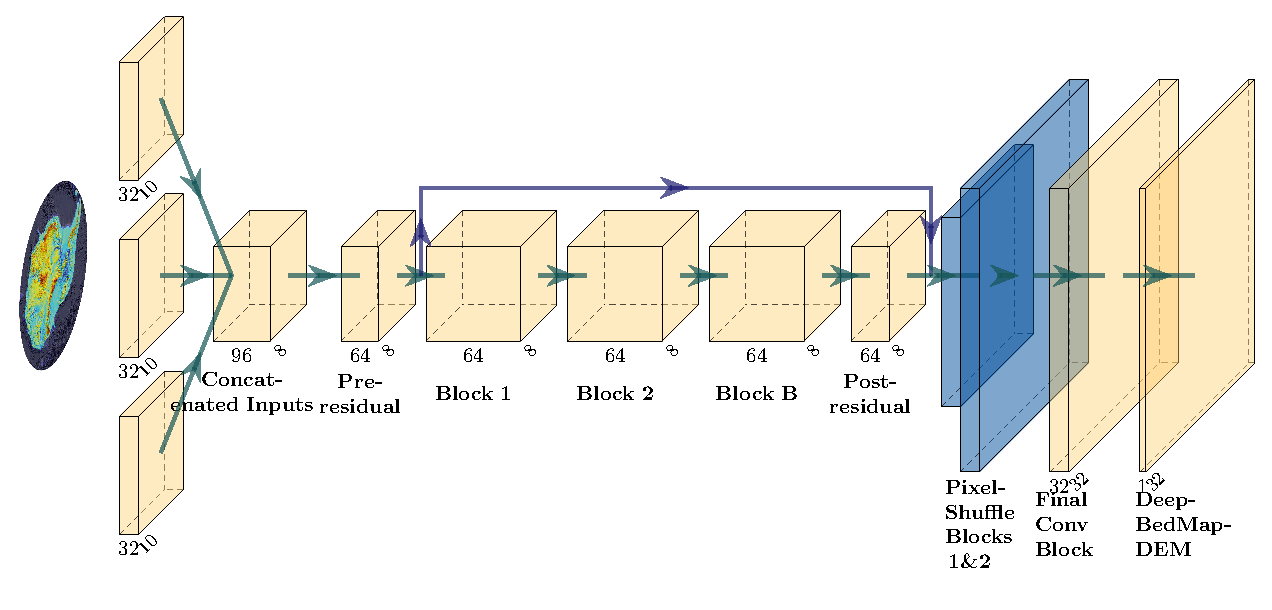
\includegraphics[width=16cm]{figures/deepbedmap_architecture.pdf}
  \caption{DeepBedMap Model Architecture}
  \label{}
\end{figure*}

Our Generative Adversarial Network model architecture is adapted from the ESRGAN model by \citet{WangESRGANEnhancedSuperResolution2018}, with a few notable differences.
Specifically, the Generator neural network model is modified to:
1) Use a custom conditional input block (see Figure 1a, focusing on input block) consisting of four sub-networks, each one having a different sized convolution size and stride so as to create identical sized outputs which are then concatenated together channel-wise before being fed into the main body of the ESRGAN-based convolutional neural network.
2) Use Deformable Convolution \citep{DaiDeformableConvolutionalNetworks2017} instead of standard Convolution in the final two layers to enhance our model's predictive capability by having it learn dense spatial transformations.

The objective of our 4 times upsampling super-resolution model is to produce a high resolution (250m) grid of Antarctica's bed elevation given a low resolution (1000m) BEDMAP2 \citep{FretwellBedmap2improvedice2013} image.
However, the information contained in BEDMAP2 is insufficient for this regular super-resolution task, so we provide the neural network with more context through network conditioning.
Specifically, the model is conditioned at the input block stage with these raster grids: 1) ice surface elevation, 2) ice surface velocity, and 3) snow accumulation, all of which are covered by satellite observations.
The non-linear relationship between the low resolution bed elevation prior (BEDMAP2) and these conditioning inputs are then processed through $B$-layers of Residual-in-Residual Dense Blocks and upsampled at the end to produce a high resolution bed elevation prediction.

This Generator model gradually improves its prediction by comparing the predicted output with the groundtruth image, specifically using the previously defined Content Loss \eqref{eq:4}, Adversarial Loss \eqref{eq:6}, Topographic Loss \eqref{eq:8}, and Structural Loss \eqref{eq:10}.
Again, we follow ESRGAN's lead in the implementation of our adversarial Discriminator network.
A VGG-style convolutional neural network \citep{SimonyanVeryDeepConvolutional2014} is used, consisting of 10 Convolutional-BatchNormalization-LeakyReLU blocks, followed by two fully connected layers with 100 and 1 neurons.
For numerical stability, the sigmoid activation output is omitted from the Discriminator model's construction and is integrated instead into the binary cross entropy loss functions \eqref{eq:5} and \eqref{eq:6} via the log-sum-exp trick.

\section{Experiments}

\subsection{Data Preparation}

Our 2D Convolutional neural network works on raster images, so we have to ensure our datasets are all in a suitable raster grid format.
Groundtruth xyz points of the bed elevation (see Table \ref{table:groundtruth}) are first compiled together onto a common Antarctic Stereographic Projection (EPSG:3031) using the WGS84 datum, reprojecting if necessary.
Using Generic Mapping Tools v6.0 \citep{WesselGenericMappingTools2019}, the points are then preprocessed using 'blockmedian' (block average using L1 norm) and gridded onto a 250m spatial resolution pixel-node registered grid using 'surface' (adjustable tension continuous curvature spline function) with a tension factor set to 0.35 and a mask set to 3 pixels (750m) from the nearest point.

To create our training dataset, we use a sliding window to obtain smaller tiles of the groundtruth grids, and also find the inputs (see Table \ref{table:datainputs}) corresponding to the same spatial bounding box area.
In order to reduce border edge effects, we have used no padding (also known as 'valid' padding) in our Generator model's input convolutional layers which means our model input grids will cover a larger spatial area than the groundtruth grids.
More specifically, the model inputs cover an area of 11x11km (e.g. 11x11pixels for BEDMAP2) while the groundtruth grids cover an area of 9x9km (36x36pixels).
As the pixels of our groundtruth grids may not align perfectly with that of our model input grids, we use bilinear interpolation to ensure that all our input grids cover the same spatial bounds as that of our reference groundtruth tiles.

\begin{table*}[h]
\caption{High Resolution groundtruth datasets from ice-penetrating radar surveys.}
\label{table:groundtruth}
\begin{tabular}{lcr}
\tophline
Location & Citation \\
\middlehline
Pine Island Glacier & \cite{BinghamDiverselandscapesPine2017} \\
Wilkes Subglacial Basin & \cite{JordanHypothesismegaoutburstflooding2010} \\
Carlson Inlet & \cite{KingIcestreamnot2011} \\
Rutford Ice Stream & \cite{KingSubglaciallandformsRutford2016} \\
Antarctica & \cite{ShiMultichannelCoherentRadar2010} \\
\bottomhline
\end{tabular}
\belowtable{} % Table Footnotes
\end{table*}

\begin{table*}[h]
\caption{Remote Sensing dataset inputs into the DeepBedMap neural network model.}
\label{table:datainputs}
\begin{tabular}{cccc}
\tophline
Symbol & Name & Spatial Resolution & Citation \\
\middlehline
$x$ & BEDMAP2 & 1000m & \cite{FretwellBedmap2improvedice2013} \\
$w^1$ & REMA & 100m* & \cite{HowatReferenceElevationModel2019} \\
$w^2$ & MEaSUREs Ice Velocity & 500m** & \cite{MouginotContinentwideinterferometric2019} \\
$w^3$ & Antarctic Snow Accumulation & 1000m & \cite{ArthernAntarcticsnowaccumulation2006} \\
\bottomhline
\end{tabular}
\belowtable{
  * gaps in 100m mosaic filled in with bilinear resampled 200m resolution REMA image \\
  ** originally 450m, bilinear resampled to 500m.
} % Table Footnotes
\end{table*}

\subsection{Training Details}

The neural networks were developed using the Chainer v7.0.0b2 \citep{TokuiChainerDeepLearning2019}, and trained using full precision (floating point 32) arithmetic.
Experiments were carried out on 4 Graphical Processing Units (GPUs), specifically 2 Tesla P100 GPUs and 2 Tesla V100 GPUs.
On our Tesla V100 GPU setup, one training run with about 150 epochs takes about 30 minutes.
This is using a batch size of 128 on a total of 3826 training image tiles, with 202 tiles reserved for validation, i.e. a 95/5 training/validation split.
We next describe the method used to evaluate each DeepBedMap candidate model, as well as the high-level way in which we semi-automatically arrived at a good model via semi-automatic hyperparameter tuning.

\begin{table*}[h]
\caption{Optimized Hyperparameter Settings.}
\label{table:1}
\begin{tabular}{lrr}
\tophline
Hyperparameter & Setting & Tuning Range \\
\middlehline
Learning rate (for both Generator and Discriminator) & 1.7e-4 & 2e-4 to 1e-4 \\
Number of Residual-in-Residual Blocks & 12 & 8 to 14 \\
Mini-batch size & 128 & 64 or 128 \\
Number of epochs & 140 & 90 to 150 \\
Residual scaling & 0.2 & 0.1 to 0.5 \\
Content Loss Weighting $\eta$ & 1e-2 & Fixed \\
Adversarial Loss Weighting $\lambda$ & 2e-2 & Fixed \\
Topographic Loss Weighting $\theta$ & 2e-3 & Fixed \\
Structural Loss Weighting $\zeta$ & 5.25 & Fixed \\
He Normal Initialization Scaling & 0.1 & Fixed \\
Adam optimizer epsilon & 0.1 & Fixed \\
Adam optimizer beta1 & 0.9 & Fixed \\
Adam optimizer beta2 & 0.99 & Fixed \\
\bottomhline
\end{tabular}
\belowtable{} % Table Footnotes
\end{table*}

To check for overfitting, we evaluate the Generative Adversarial Network model on our validation dataset after each epoch using two performance metrics - a peak signal-to-noise ratio (PSNR) metric for the Generator, and an accuracy metric for the Discriminator.
Training stops when these validation performance metrics show little improvement, roughly at 90 epochs.

Next, we conduct a full evaluation on an independent test dataset, comparing the model's predicted grid output against actual groundtruth xyz points.
Using the 'grdtrack' function in Generic Mapping Tools v6.0 \citep{WesselGenericMappingTools2019}, we obtain the grid elevation at each of our groundtruth point and use it to calculate the elevation error on a point-to-point basis.
All of these elevation errors are then used to compute a Root Mean Squared Error (RMSE) statistic over this independent test site.
This RMSE value is used to judge our model's performance in relation to baseline bicubic interpolation, and also the metric minimized by our hyperparameter optimization algorithm which we will describe next.

Neural networks contain a lot of hyperparameter settings that need to be decided upon, and Generative Adversarial Networks are particularly sensitive to different hyperparameter settings.
To stabilize model training and obtain better performance, we tune our hyperparameters (see Table \ref{table:1}) using a bayesian approach.
Specifically, we employ the Tree-structured Parzen Estimator \citep{BergstraAlgorithmsHyperparameterOptimization2011} from the Optuna v0.14.0 \citep{AkibaOptunaNextgenerationHyperparameter2019} with default settings as per the Hyperopt library \citep{BergstraHyperoptPythonlibrary2015}.
Given that we have 4 GPUs, we choose to parallelize the hyperparameter tuning experiments asynchronously between all four devices.
The estimator first conducts 20 random experimental trials to scan the hyperparameter space, gradually narrowing down to a few candidate hyperparameters in subsequent experiments.
We set each GPU to run a target of 30 experimental trials (i.e. a total of 120), though unpromising trials that have exploding/vanishing gradients are pruned prematurely to save on time and computational resources.
Finally, we present our results in the next section, comparing our DeepBedMap DEM grid with surfaces produced by other methods.


\section{Discussion}

Our DeepBedMap convolutional neural network method presents a purely data-driven approach to resolve the bed topography of Antarctica.
It is an improvement beyond simple interpolation techniques, generating realistic high spatial resolution (250m) topography that preserves details in bed roughness and is adaptable for catchment to continent-scale studies.
The method's GPU-based training and inference allows it to scale easily, performing better with the addition of more training datasets.
Unlike other inverse methods that rely on some explicit paramerization of ice-flow physics, our model uses deep learning to find suitable neural network parameters via an iterative error minimization approach.

In the results section, we quantify that the DeepBedMap neural network model can produce a lower error than existing interpolation and inverse modelling efforts in some circumstances.
Our DeepBedMap\_DEM v1 has established a high resolution topographic result about halfway between the groundtruth surface and bicubic interpolated surface, which can be taken as the current empirical best for an inverse topographic model(?).
Note however, that the topography generated by our model is quite sensitive to the accuracy of its inputs, and though this is a problem faced by many other inverse methods, neural network models like ours can be particularly biased towards the training dataset.
In particular, our experimental model's topography is likely skewed towards the distribution of our training regions that tend to reside in coastal regions, especially over West Antarctica (see training regions figure).

Moving forward, we have identified a strong need for better quality datasets over many parts of Antarctica.
Our DeepBedMap model is trained only on a small fraction of the area of Antarctica, simply because the Convolutional Neural Network can't be trained on sparse survey point measurements.
There is a need for denser, high resolution surveys (<250m flight spacing) that capture a more representative picture of Antarctica's varied bed topography.
Also, some of the conditional datasets we use such as REMA \citep{HowatReferenceElevationModel2019} and MEaSUREs Ice Velocity \citep{RignotMEaSUREsInSARBasedAntarctica2017} have data gaps which introduce artifacts in the DeepBedMap\_DEM, and those need to be filled up properly for continent-wide prediction.
Another limitation is that the DeepBedMap model currently relies on snapshot data collected over different epochs and has no proper sense of time.
Ice Elevation Change (e.g. from ICESat-2 \citep{MarkusIceCloudland2017}) could be an additional input to better account for this and could further improve the model's performance.

The work here is not meant to discourage use of hand designed inverse modelling technique, but to introduce an independent methodology, with an outlook towards combining the strengths of the two to provide an even more accurate bed elevation map of Antarctica.
One side product resulting from this work is a test-driven development framework that can be used to measure and compare the performance of upcoming bed terrain models.
Indeed, the radioglaciology community has begun to compile a more comprehensive bed elevation/ice thickness dataset for Antarctica, and there has been some discussion to combine various terrain interpolation techniques in an ensemble to create BEDMAP3.

\conclusions  %% \conclusions[modified heading if necessary]
TEXT

%% The following commands are for the statements about the availability of data sets and/or software code corresponding to the manuscript.
%% It is strongly recommended to make use of these sections in case data sets and/or software code have been part of your research the article is based on.

\codeavailability{TEXT} %% use this section when having only software code available


\dataavailability{TEXT} %% use this section when having only data sets available


\codedataavailability{TEXT} %% use this section when having data sets and software code available


\sampleavailability{TEXT} %% use this section when having geoscientific samples available


\videosupplement{TEXT} %% use this section when having video supplements available


\appendix
\section{}    %% Appendix A

\subsection{}     %% Appendix A1, A2, etc.


\noappendix       %% use this to mark the end of the appendix section

%% Regarding figures and tables in appendices, the following two options are possible depending on your general handling of figures and tables in the manuscript environment:

%% Option 1: If you sorted all figures and tables into the sections of the text, please also sort the appendix figures and appendix tables into the respective appendix sections.
%% They will be correctly named automatically.

%% Option 2: If you put all figures after the reference list, please insert appendix tables and figures after the normal tables and figures.
%% To rename them correctly to A1, A2, etc., please add the following commands in front of them:

\appendixfigures  %% needs to be added in front of appendix figures

\appendixtables   %% needs to be added in front of appendix tables

%% Please add \clearpage between each table and/or figure. Further guidelines on figures and tables can be found below.



\authorcontribution{TEXT} %% this section is mandatory

\competinginterests{TEXT} %% this section is mandatory even if you declare that no competing interests are present

\disclaimer{TEXT} %% optional section

\begin{acknowledgements}
TEXT
\end{acknowledgements}




%% REFERENCES

%% The reference list is compiled as follows:

%% \begin{thebibliography}{}

%% \bibitem[AUTHOR(YEAR)]{LABEL1}
%% REFERENCE 1

%% \bibitem[AUTHOR(YEAR)]{LABEL2}
%% REFERENCE 2

%% \end{thebibliography}

%% Since the Copernicus LaTeX package includes the BibTeX style file copernicus.bst,
%% authors experienced with BibTeX only have to include the following two lines:
%%
\bibliographystyle{copernicus}
\bibliography{example.bib}
%%
%% URLs and DOIs can be entered in your BibTeX file as:
%%
%% URL = {http://www.xyz.org/~jones/idx_g.htm}
%% DOI = {10.5194/xyz}


%% LITERATURE CITATIONS
%%
%% command                        & example result
%% \citet{jones90}|               & Jones et al. (1990)
%% \citep{jones90}|               & (Jones et al., 1990)
%% \citep{jones90,jones93}|       & (Jones et al., 1990, 1993)
%% \citep[p.~32]{jones90}|        & (Jones et al., 1990, p.~32)
%% \citep[e.g.,][]{jones90}|      & (e.g., Jones et al., 1990)
%% \citep[e.g.,][p.~32]{jones90}| & (e.g., Jones et al., 1990, p.~32)
%% \citeauthor{jones90}|          & Jones et al.
%% \citeyear{jones90}|            & 1990



%% FIGURES

%% When figures and tables are placed at the end of the MS (article in one-column style), please add \clearpage
%% between bibliography and first table and/or figure as well as between each table and/or figure.


%% ONE-COLUMN FIGURES

%%f
%\begin{figure}[t]
%\includegraphics[width=8.3cm]{FILE NAME}
%\caption{TEXT}
%\end{figure}
%
%%% TWO-COLUMN FIGURES
%
%%f
%\begin{figure*}[t]
%\includegraphics[width=12cm]{FILE NAME}
%\caption{TEXT}
%\end{figure*}
%
%
%%% TABLES
%%%
%%% The different columns must be seperated with a & command and should
%%% end with \\ to identify the column brake.
%
%%% ONE-COLUMN TABLE
%
%%t
%\begin{table}[t]
%\caption{TEXT}
%\begin{tabular}{column = lcr}
%\tophline
%
%\middlehline
%
%\bottomhline
%\end{tabular}
%\belowtable{} % Table Footnotes
%\end{table}
%
%%% TWO-COLUMN TABLE
%
%%t
%\begin{table*}[t]
%\caption{TEXT}
%\begin{tabular}{column = lcr}
%\tophline
%
%\middlehline
%
%\bottomhline
%\end{tabular}
%\belowtable{} % Table Footnotes
%\end{table*}
%
%%% LANDSCAPE TABLE
%
%%t
%\begin{sidewaystable*}[t]
%\caption{TEXT}
%\begin{tabular}{column = lcr}
%\tophline
%
%\middlehline
%
%\bottomhline
%\end{tabular}
%\belowtable{} % Table Footnotes
%\end{sidewaystable*}
%
%
%%% MATHEMATICAL EXPRESSIONS
%
%%% All papers typeset by Copernicus Publications follow the math typesetting regulations
%%% given by the IUPAC Green Book (IUPAC: Quantities, Units and Symbols in Physical Chemistry,
%%% 2nd Edn., Blackwell Science, available at: http://old.iupac.org/publications/books/gbook/green_book_2ed.pdf, 1993).
%%%
%%% Physical quantities/variables are typeset in italic font (t for time, T for Temperature)
%%% Indices which are not defined are typeset in italic font (x, y, z, a, b, c)
%%% Items/objects which are defined are typeset in roman font (Car A, Car B)
%%% Descriptions/specifications which are defined by itself are typeset in roman font (abs, rel, ref, tot, net, ice)
%%% Abbreviations from 2 letters are typeset in roman font (RH, LAI)
%%% Vectors are identified in bold italic font using \vec{x}
%%% Matrices are identified in bold roman font
%%% Multiplication signs are typeset using the LaTeX commands \times (for vector products, grids, and exponential notations) or \cdot
%%% The character * should not be applied as mutliplication sign
%
%
%%% EQUATIONS
%
%%% Single-row equation
%
%\begin{equation}
%
%\end{equation}
%
%%% Multiline equation
%
%\begin{align}
%& 3 + 5 = 8\\
%& 3 + 5 = 8\\
%& 3 + 5 = 8
%\end{align}
%
%
%%% MATRICES
%
%\begin{matrix}
%x & y & z\\
%x & y & z\\
%x & y & z\\
%\end{matrix}
%
%
%%% ALGORITHM
%
%\begin{algorithm}
%\caption{...}
%\label{a1}
%\begin{algorithmic}
%...
%\end{algorithmic}
%\end{algorithm}
%
%
%%% CHEMICAL FORMULAS AND REACTIONS
%
%%% For formulas embedded in the text, please use \chem{}
%
%%% The reaction environment creates labels including the letter R, i.e. (R1), (R2), etc.
%
%\begin{reaction}
%%% \rightarrow should be used for normal (one-way) chemical reactions
%%% \rightleftharpoons should be used for equilibria
%%% \leftrightarrow should be used for resonance structures
%\end{reaction}
%
%
%%% PHYSICAL UNITS
%%%
%%% Please use \unit{} and apply the exponential notation


\end{document}
